\documentclass[12pt]{article}
\usepackage{amsmath, amsthm, amssymb}
\usepackage{hyperref}
\usepackage[top=1.0in, bottom=1.0in, left=1.0in, right=1.0in]{geometry}
\usepackage{hyperref}
\usepackage{mathscinet}
\usepackage{tikz,tkz-graph,tkz-berge}
\usetikzlibrary{positioning}
\usepackage{verbatim, xcolor}

\usetikzlibrary{arrows}
\usetikzlibrary{decorations.markings}
\newcommand{\boundellipse}[3]% center, xdim, ydim
{(#1) ellipse (#2 and #3)
}

\pagestyle{plain}

\usepackage{sectsty}
\allsectionsfont{\sffamily}

\setcounter{secnumdepth}{5}
\setcounter{tocdepth}{5}

\makeatletter
\newtheorem*{rep@theorem}{\rep@title}
\newcommand{\newreptheorem}[2]{
\newenvironment{rep#1}[1]{
 \def\rep@title{#2 \ref{##1}}
 \begin{rep@theorem}}
 {\end{rep@theorem}}}
\makeatother

\theoremstyle{plain}
\newtheorem{thm}{Theorem}[section]
\newreptheorem{thm}{Theorem}
\newtheorem{prop}[thm]{Proposition}
\newreptheorem{prop}{Proposition}
\newtheorem{lem}[thm]{Lemma}
\newreptheorem{lem}{Lemma}
\newtheorem{conjecture}[thm]{Conjecture}
\newreptheorem{conjecture}{Conjecture}
\newtheorem{cor}[thm]{Corollary}
\newreptheorem{cor}{Corollary}
\newtheorem{prob}[thm]{Problem}

\newtheorem*{Theorem}{Theorem}
\newtheorem*{Lemma}{Lemma}


\theoremstyle{definition}
\newtheorem{defn}{Definition}
\theoremstyle{remark}
\newtheorem*{remark}{Remark}
\newtheorem*{problem}{Problem}
\newtheorem{example}{Example}
\newtheorem*{question}{Question}
\newtheorem*{observation}{Observation}

\newcommand{\fancy}[1]{\mathcal{#1}}
\newcommand{\C}[1]{\fancy{C}_{#1}}
\newcommand{\IN}{\mathbb{N}}
\newcommand{\IR}{\mathbb{R}}
\newcommand{\G}{\fancy{G}}
\newcommand{\CC}{\fancy{C}}
\newcommand{\D}{\fancy{D}}
\newcommand{\T}{\fancy{T}}
\newcommand{\B}{\fancy{B}}
\renewcommand{\L}{\fancy{L}}
\newcommand{\HH}{\fancy{H}}

\newcommand{\inj}{\hookrightarrow}
\newcommand{\surj}{\twoheadrightarrow}

\newcommand{\set}[1]{\left\{ #1 \right\}}
\newcommand{\setb}[3]{\left\{ #1 \in #2 \mid #3 \right\}}
\newcommand{\setbs}[2]{\left\{ #1 \mid #2 \right\}}
\newcommand{\card}[1]{\left|#1\right|}
\newcommand{\size}[1]{\left\Vert#1\right\Vert}
\newcommand{\ceil}[1]{\left\lceil#1\right\rceil}
\newcommand{\floor}[1]{\left\lfloor#1\right\rfloor}
\newcommand{\func}[3]{#1\colon #2 \rightarrow #3}
\newcommand{\funcinj}[3]{#1\colon #2 \inj #3}
\newcommand{\funcsurj}[3]{#1\colon #2 \surj #3}
\newcommand{\irange}[1]{\left[#1\right]}
\newcommand{\join}[2]{#1 \mbox{\hspace{2 pt}$\ast$\hspace{2 pt}} #2}
\newcommand{\djunion}[2]{#1 \mbox{\hspace{2 pt}$+$\hspace{2 pt}} #2}
\newcommand{\parens}[1]{\left( #1 \right)}
\newcommand{\brackets}[1]{\left[ #1 \right]}
\newcommand{\DefinedAs}{\mathrel{\mathop:}=}

\newcommand{\mic}{\operatorname{mic}}
\newcommand{\AT}{\operatorname{AT}}
\newcommand{\col}{\operatorname{col}}
\newcommand{\ch}{\operatorname{ch}}

\newcommand{\erdos}{Erd\H{o}s}
\newcommand{\CondOne}{\hyperref[cond1]{Condition (1)}}
\newcommand{\CondTwo}{\hyperref[cond2]{Condition (2)}}

\def\adj{\leftrightarrow}
\def\nonadj{\not\!\leftrightarrow}

\newcommand\restr[2]{{% we make the whole thing an ordinary symbol
  \left.\kern-\nulldelimiterspace % automatically resize the bar with \right
  #1 % the function
  \vphantom{\big|} % pretend it's a little taller at normal size
  \right|_{#2} % this is the delimiter
  }}

\def\D{\fancy{D}}
\def\C{\fancy{C}}
\def\A{\fancy{A}}
\def\L{\fancy{L}}
\def\H{\fancy{H}}

\newcommand{\case}[2]{{\bf Case #1.}~{\it #2}~~}
\newcommand{\claim}[2]{{\bf Claim #1.}~{\it #2}~~}
\newcommand{\subclaim}[2]{{\bf Subclaim #1.}~{\it #2}~~}

\title{graph theory notes\thanks{clarifications, errors, simplifications $\Rightarrow$ \texttt{landon.rabern@gmail.com}}\\ \bigskip
The union of a forest and a star forest is $3$-colorable}
\date{}
\begin{document}
\maketitle
Norbert Sauer conjectured the following in 1993 \cite{sauer} and Michael Stiebitz proved it in 1994 \cite{stiebitz1994forest}.  A \emph{star forest} is a forest where each component has a dominating vertex called the \emph{root}.
It is easy to see that for two forests $F_1$ and $F_2$ we have $\chi(F_1 \cup F_2) \le 4$.  We can do better when one of the forests is a star forest.
\begin{Theorem}[Stiebitz]
If $F_1$ is a star forest and $F_2$ is a forest, then $\chi(F_1 \cup F_2) \le 3$.
\end{Theorem}

In fact, Stiebitz proved a stronger statement.  Theorem follows immediately by applying Lemma with $k=3$, $F = F_2$ and $H$ the subgraph of $G$ induced on the set of roots of $F_1$.  The following proof and picture are from the paper \emph{Brooks' Theorem and Beyond} with Dan Cranston \cite{brooksbeyond}.

\begin{Lemma}[Stiebitz]
\label{stiebitz}
Let $H$ be an induced subgraph of a graph $G$ with $\chi(H) \le k$ for some $k \ge 3$.  Then $\chi(G) \le k$ if $G$ has a spanning forest $F$ where
\begin{enumerate}
\item for each component $C$ of $H$, $F\brackets{V(C)}$ is a tree; and
\label{cond1}
\item $d_G(v) \le d_F(v) + k-2$ for every $v \in V(G-H)$.
\label{cond2}
\end{enumerate}
\end{Lemma}
\begin{proof}
For any graphs $U$ and $W$, we write $U-W$ for the subgraph of $U$ induced by
$V(U)\setminus V(W)$.
If $uv\in E(F)$, then $u$ is an \emph{$F$-neighbor} of $v$, and $u$ and $v$ are
\emph{$F$-adjacent}.
Suppose the lemma is false and choose a counterexample pair $G, H$ minimizing
$|G-H|$.
Note that each vertex $v$ in $G-H$ must have a neighbor in $H$, since 
otherwise we can add $v$ to $H$.  Thus $\card{H}\ge 1$.

\textbf{Claim 1.} \textit{If there exists $v \in V(G-H)$ adjacent to
components $A_1, \ldots, A_s$ of $H$ with $d_G(v) \le s + k - 2$, then there
exist $i$ and $j$, with $i \ne j$, and a path in $F-v$ from $A_i$ to $A_j$.}
Suppose not and choose such a $v \in V(G-H)$.  
We will find a $k$-coloring of $G$.
For each $i \in \irange{s}$, let $z_i$ be a neighbor of $v$ in $A_i$.  Form
$G'$, $F'$, $H'$ from $G$, $F$, $H$ (repectively) by deleting $v$ and
identifying all $z_i$ as a single new vertex $z$.  
Now $\chi(H') \le k$, since by permuting colors in each component we can get
a $k$-coloring of $H$ where all the $z_i$ use the same color.  Also, $F'$ is a
spanning forest in $G'$ since we are assuming there is no path in $F-v$ from
$A_i$ to $A_j$ whenever $i \ne j$.  It is easy to check that Conditions 
\hyperref[cond1]{(1)} and \hyperref[cond2]{(2)} hold for $G', F', H'$.  Now
$|G'-H'|<|G-H|$, so by minimality of $|G-H|$,
we have a $k$-coloring of $G'$.  This gives a $k$-coloring of $G-v$ where $z_1,
\ldots, z_s$ all get the same color.  So $v$ has at most $d_G(v) - (s-1) \le
k-1$ colors used on its neighborhood, leaving a color free to finish the
$k$-coloring on $G$, a contradiction.

\begin{center}
\begin{figure}

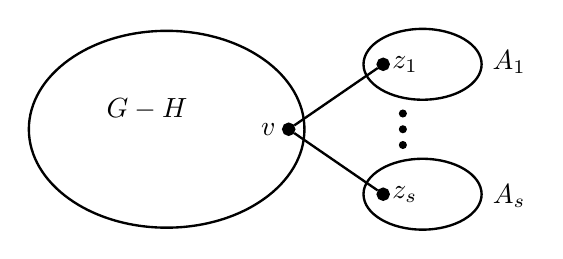
\begin{tikzpicture}[line width=.03cm,scale=.5] % start of left picture
\tikzstyle{vert}=[draw,shape=circle,fill=black,minimum size=4pt, inner sep=0pt] 
\tikzstyle{small}=[draw,shape=circle,fill=black,minimum size=2pt, inner sep=0pt] 

\draw \boundellipse{-4,0}{3.5}{2.5}; % big oval left
\draw (-.9,0) node[vert,label={[label distance=-.05cm]180:{$v$}}] (v) {}; % v
\draw (-4.5,.5) node (GminusH) {$G-H$}; % G-H

\draw \boundellipse{2.5,1.65}{1.5}{.9}; % small oval top right
\draw (4.7,1.7) node (A1) {$A_1$}; % A1
\draw (1.5,1.65) node[vert,label={[label distance=-.1cm]0:{$z_1$}}] (z1) {}; % z1 

\draw \boundellipse{2.5,-1.65}{1.5}{.9}; % small oval bottom right
\draw (4.7,-1.7) node (As) {$A_s$}; % As
\draw (1.5,-1.65) node[vert,label={[label distance=-.1cm]0:{$z_s$}}] (zs) {}; % zs 

% small dots between z1 and zs
\draw (z1) -- (v) -- (zs);
\draw (2.0,.4) node[small] () {};
\draw (2.0,0) node[small] () {};
\draw (2.0,-.4) node[small] () {};
% \draw (-6,-2.8) -- (6,-2.8); % straight rule
\end{tikzpicture}
%\bigskip
%
%\bigskip
\hspace{.25in}
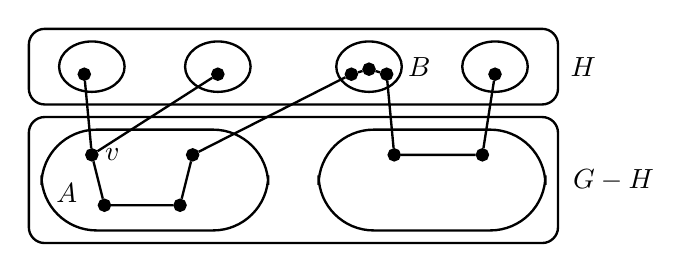
\begin{tikzpicture}[line width=.03cm,scale=.32] % start of right picture
\tikzstyle{vert}=[draw,shape=circle,fill=black,minimum size=4pt, inner sep=0pt] 

% two left ovals
\draw \boundellipse{-6,.5}{1.3}{1};
\draw (-6.3,.2) node[vert] (u1) {}; % u1
\draw \boundellipse{-1,.5}{1.3}{1};
\draw (-1,.2) node[vert] (u2) {}; % u2

% left box
\draw[rounded corners=.7cm] (-8,-2) -- (-8,-6) -- (1,-6) -- (1,-2) -- cycle;
%\draw (-6,-3) node[vert] (v) {}; % v
\draw (-6,-3) node[vert,label={[label distance=-.05cm]360:{$v$}}] (v) {}; % v
\draw (-5.5,-5) node[vert] (v2) {}; % v2
\draw (-2.5,-5) node[vert] (v3) {}; % v3
\draw (-2,-3) node[vert] (v4) {}; % v4
\draw (u1) -- (v) -- (v2) -- (v3) -- (v4) (u2) -- (v);

\begin{scope}[xshift=11cm] % right side

\draw \boundellipse{-6,.5}{1.3}{1};
\draw (-6.7,.2) node[vert] (u3) {}; % u3
\draw (-6.0,.4) node[vert] (u4) {}; % u4 
\draw (-5.3,.2) node[vert] (u5) {}; % u5
\draw \boundellipse{-1,.5}{1.3}{1};
\draw (-1,.2) node[vert] (u6) {}; % u6

\draw[rounded corners=.7cm] (-8,-2) -- (-8,-6) -- (1,-6) -- (1,-2) -- cycle;

\draw (-5.0,-3) node[vert] (v5) {}; % v5
\draw (-1.5,-3) node[vert] (v6) {}; % v6
\draw (v4) -- (u3) -- (u4) -- (u5) -- (v5) -- (v6) -- (u6);
\end{scope}

\draw[rounded corners=.2cm] (-8.5,-1.5) -- (-8.5,-6.5) -- (12.5,-6.5) --
(12.5,-1.5) -- cycle; % Box for G-H
\draw[rounded corners=.2cm] (-8.5,-1) -- (-8.5,2) -- (12.5,2) --
(12.5,-1) -- cycle; % Box for H

\draw (14.7,-4) node[] (GminusH) {$G-H$}; % G-H
\draw (13.5,.5) node[] (H) {$H$}; % H
\draw (7.0,.5) node[] (B) {$B$}; % B
\draw (-7,-4.5) node[] (A) {$A$}; % A
\end{tikzpicture}

\caption{The left figure shows Claim 1. The right figure 
shows Claim 3.
}
\label{lemma7-figs}
\end{figure}
\end{center}

\textbf{Claim 2.} \textit{Every leaf of $F$ is in $H$ and every vertex not in
$H$ has an $F$-neighbor not in $H$.}
We can rewrite this formally: $d_F(v) \ge 2$ and $d_{F-H}(v) \ge 1$ for all $v
\in V(G-H)$.
Applying Claim 1 with $s=1$ implies $d_G(v) \ge k$. 
Now {\CondTwo} gives $d_F(v) \ge d_G(v) + 2 - k \ge 2$. Suppose
$d_{F-H}(v) = 0$ for some $v \in V(G-H)$.   Since $F$ is a forest, {\CondOne} 
implies that all $F$-neighbors of $v$ must be in different components of $H$.
Moreover there can be no path between two of these components in $F-v$.  
{\CondTwo} gives $d_G(v)\le d_F(v)+k-2$, so
applying Claim 1 with $s = d_F(v)$ gives a contradiction.
Thus $d_{F-H}(v) \ge 1$ for all $v\in V(G-H)$.

\textbf{Claim 3.} 
\textit{There exists $v$ in $G-H$ with $d_{F-H}(v) = 1$ such that every
component of $H$ that is $F$-adjacent to $v$ is not $F$-adjacent to any other
vertex in $G-H$.}
Form a bipartite graph $F'$ from $F$ by contracting each component of $H$ and
each component of $F-H$ to a single vertex.  Since $F$ is a forest, {\CondOne}
implies that $F'$ is also a forest.  So some vertex contracted from a component
$A$ of $F-H$ has at most one neighbor of degree at least 2; say this neighbor
is contracted from $B$, where $B\subseteq (F\cap H)$.  (If not, then we can
walk between components of $H$ and $F-H$ until we get a cycle in $F$.)
Let $v$ be a leaf of $A$ that is not $F$-adjacent to $B$; this gives
$d_{F-H}(v) = d_{A}(v)\le 1$.  Claim 2 gives $d_{F-H}(v)\ge 1$, so in fact
$d_{F-H}(v)=1$ as desired.

\textbf{Claim 4.} \textit{If the $v$ in Claim 3 is adjacent to a component of
$H$, then it is $F$-adjacent to that component.}
Let $A_1, \ldots, A_r$ be the components of $H$ that are $F$-adjacent to $v$,
where $r = d_F(v) - 1$.  Suppose there is another component $A_{r+1}$ of $H$
that is adjacent to $v$.  Since no vertex of $G-H$ besides $v$ is $F$-adjacent
to any of $A_1, \ldots, A_r$, there can be no $F$-path in $F-v$ between any
pair among $A_1, \ldots, A_r, A_{r+1}$.  Now the contrapositive of Claim 1
implies that $d_G(v) > (r + 1) + k - 2 = d_F(v) + k - 2$; this inequality
contradicts {\CondTwo}.

\textbf{Claim 5.} \textit{The lemma holds.}
Let $H' \DefinedAs G[V(H) \cup \set{v}]$, with $v$ as in Claims 3 and 4.  
By Claim 4, {\CondOne} of the
hypotheses holds for $H'$. {\CondTwo} clearly holds and $F$ is still a forest. Also, by permuting colors in the components we can get a $k$-coloring of $H$ where all $F$-neighbors of $v$ get the same color.  Hence $v$ has at most $d_H(v) - (d_F(v) - 2) \le d_G(v) - 1 - (d_F(v) - 2) = d_G(v) - d_F(v) + 1 \le k-1$ colors on its neighborhood.  Hence $H'$ is $k$-colorable. But then, by minimality of $|G-H|$, $G$ is $k$-colorable, a contradiction.
\end{proof}

Combined with a result on the existence of spanning trees with pairwise non-adjacent leaves \cite{independencytree}, Lemma yields Brooks' theorem \cite{brooks1941colouring}.  See \cite{brooksbeyond} for details.

\begin{question}
Are there other applications of Lemma?
\end{question}

\bibliographystyle{amsplain}
\bibliography{GraphColoring}
\end{document}

 
